\documentclass[a4, 11pt]{article}
\usepackage[utf8]{inputenc}
\usepackage[a4paper,bindingoffset=0.2in,%
 left=0.5in,right=0.5in,top=1in,bottom=1in,%
            footskip=.25in]{geometry}
\usepackage{cite}
\usepackage[english]{babel}
\usepackage{graphicx}
\usepackage{caption}
\usepackage{subfigure}
\usepackage{hyperref}
\setlength{\parskip}{1em}
\renewcommand{\baselinestretch}{1.0}
\setlength{\parindent}{0pt}

\title{
  \textbf{Investigating and Modeling of the Correlation of COVID Cases and Regional Features based on Local Government Area in Victoria}\\
  }
\author{Xuanxiu Chen,Ziming Wang, Chengyi Huang, Min Zhang}
\date{}


\begin{document}
\thispagestyle{empty}
    \begin{center}
    \parbox[t][1cm][t]{\textwidth}{
    \begin{center}  \end{center} }


    \parbox[t][13cm][c]{\textwidth}{\huge
    \begin{center} {\textbf{\textsf Investigating and Modeling of the Correlation of COVID Cases and Regional Features based on Local Government Area in Victoria }}\end{center} }


    \parbox[t][3cm][b]{\textwidth}{
    \begin{center} {\large{\textbf{Xuanxiu Chen, Ziming Wang, Chengyi Huang, Min Zhang} }} \end{center} }
 \begin{center} https://github.com/COMP20008/assignment-2-comp20008-ass2-group-69\end{center}
    \parbox[t][2cm][c]{\textwidth}{ {\large
    \begin{center}
      University of Melbourne
    \end{center}}
\begin{center} {\textbf COMP20008 Element of data processing}\end{center} }

    \parbox[t][2cm][b]{\textwidth}{
    \begin{center} {\large\textbf{\textsf 15th October 2021}} \end{center} }
    \end{center}

\newpage
\section{Introduction}
\begin{figure}[h]
    \centering
    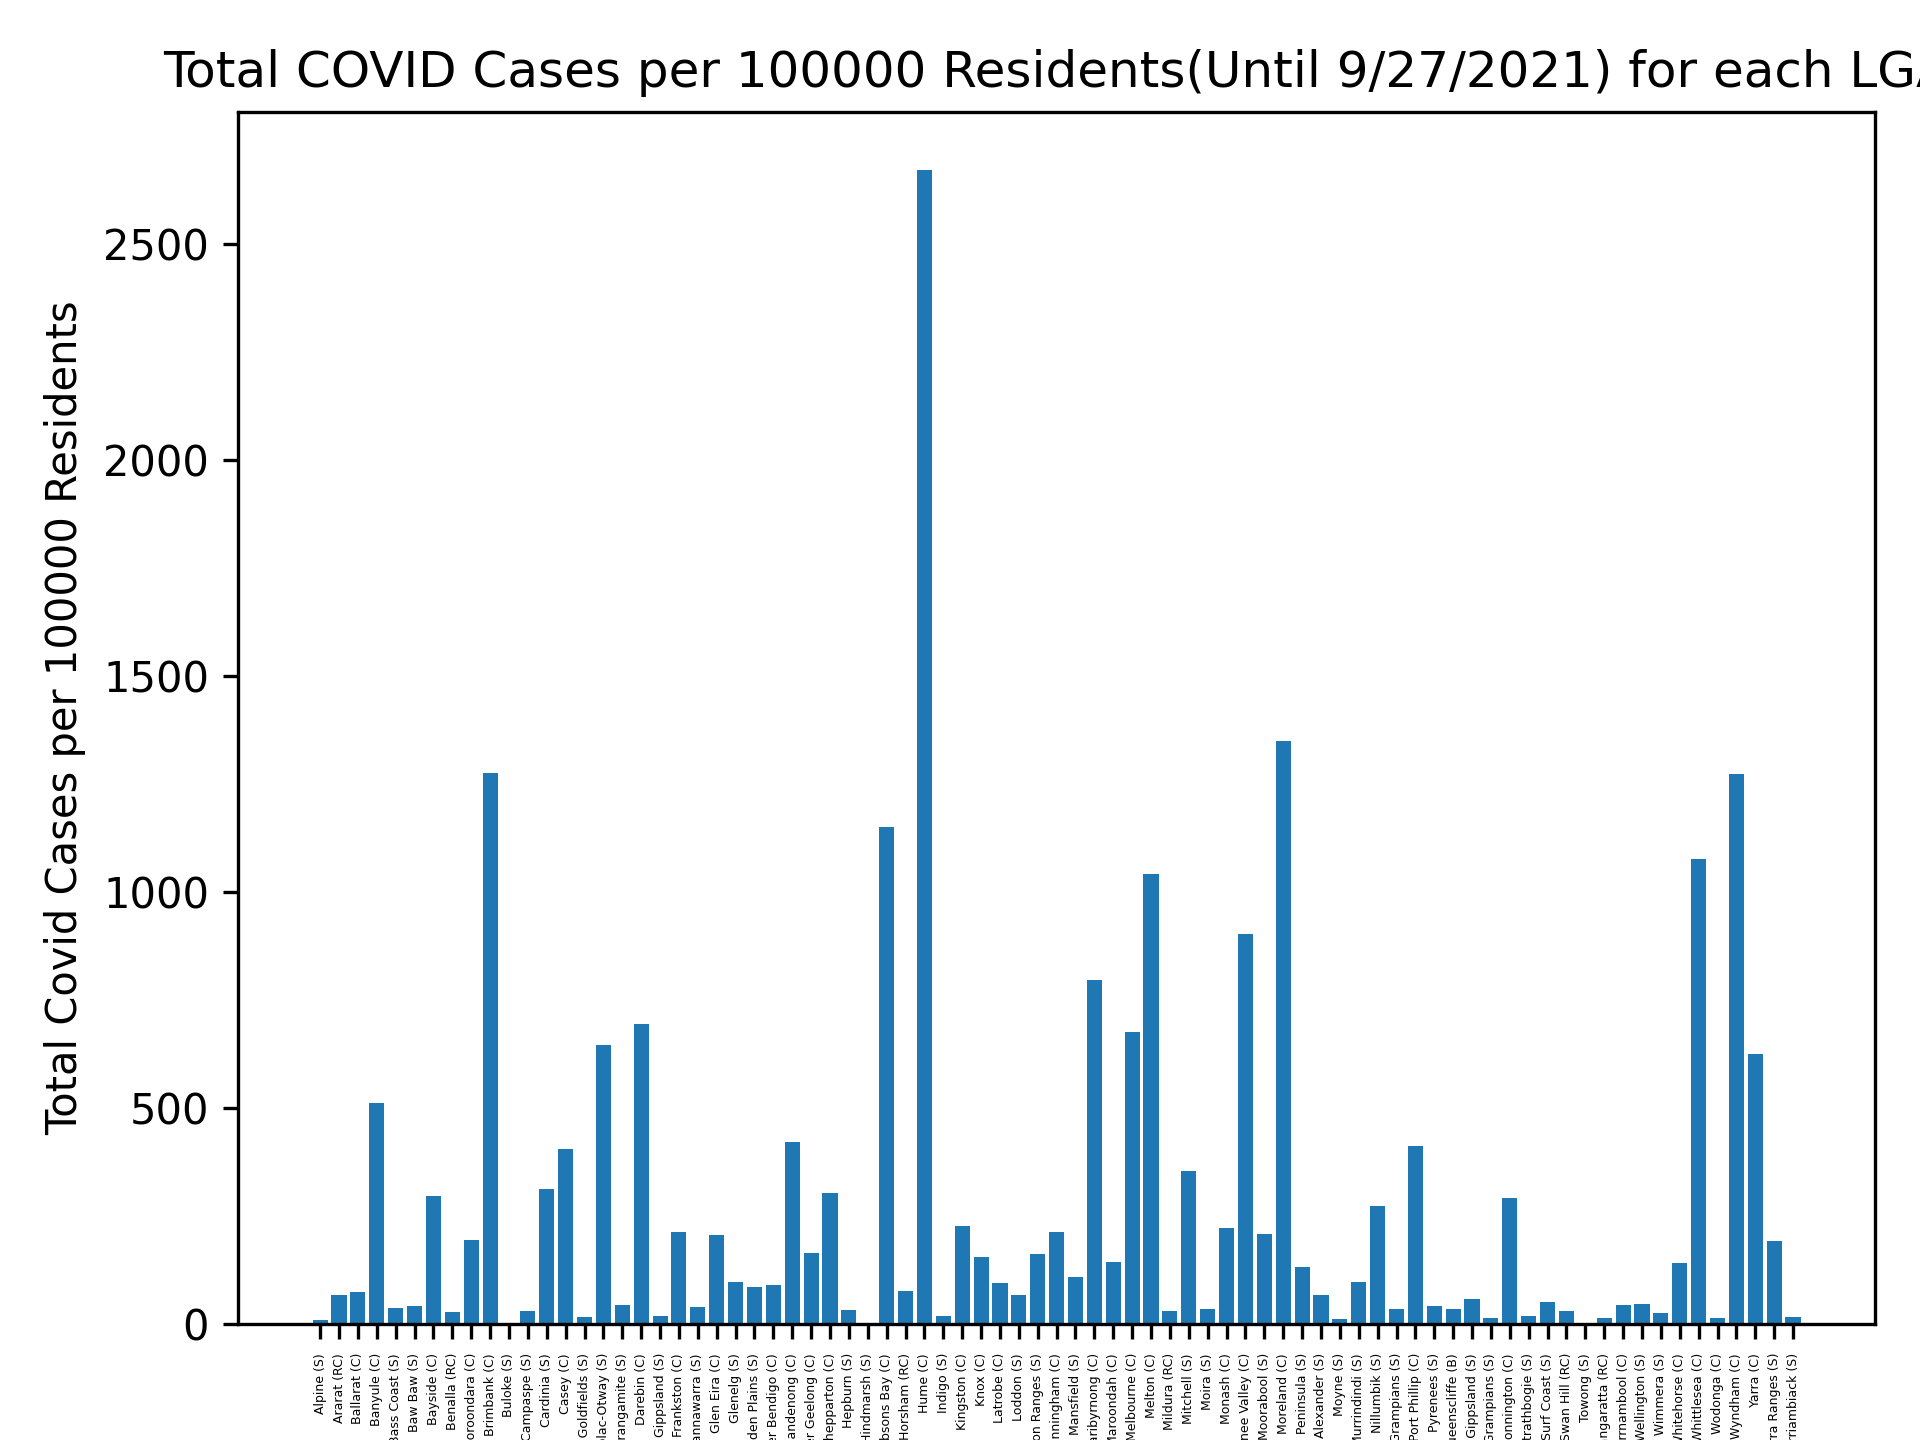
\includegraphics[width=0.7\textwidth]{graph/covidBarChart.png}
    \caption{COVID rate by Local Government Area in Victoria}
    \label{fig:my_label}
\end{figure}

The outbreak of Coronavirus not only continues to deteriorate the public health of Victorian residents, but also puts a heavy financial burden on the Victorian government due to the measures in response to the pandemic. For a long period of time, the Victorian government handled their response in a context of uncertainty. It’s important to understand why different suburbs have been hit differently in the pandemic (as shown in Figure 1) by evaluating the correlation between severity of COVID cases and the asymmetric regional features in the aspects of health and social factors. For this purpose, the research question of our project is what are the regional features (population density, domestic traveling volume, crime rate, vaccination rate) that may influence the spread of COVID across different Local Government Areas in Victoria? As a research group, we aim to help the Victorian government to make differentiated territorial policies that most accurately tackle the issues of each specific Local Government Areas (LGA) that share common properties.

\section{Data Sets Used}
Our main measurement is the number of COVID cases released by Victorian officials on a daily basis. Other numerical datasets for our four targeting regional features (population density, domestic travelling volume, community safety, vaccination rate) was collected from a variety of sources including Australian Bureau of Statistics, Crime Statistic Agency and a non-official website called COVIDLIVE to obtain the everyday vaccination rate by LGA. The obtained forms were in varieties such as xls., csv. and web page, where each dataset was linked by the LGA. The COVID confirmed cases and vaccination rate data was collected on 27th September 2021. Other Crime incident data was recorded by March 2021; population density was calculated from the data of 2019-2020; LGA internal arrival value was published by 2019.


\section{Wrangling and Analysis Methods}
For data preprocessing, a combination of manual removal and Python based automated process was employed. Furthermore, sorting functions were used on “LGA” to achieve data linkage. Outlier removal was performed to further pre-process the data to get it the optimal result.
\\A scatter plot for each individual regional feature was drawn after data were cleaned. The choice of scatter plot over any other plots was due to the nature that we have two numerical columns from one plot.
\\In addition, we calculated the NMI (normalized mutual information) and Pearson correlation coefficient to further investigate the correlation between number of covid cases and regional features.
\\Then, by feature filtering based on the NMI and Pearson correlation, we chose the most valuable features as our model input data. Then we conducted supervised machine learning techniques including classification and linear regression to build our model and calculate the accuracy.



\section{Results}
\subsection{Outlier Removal}
\begin{figure}[ht]
    \centering
    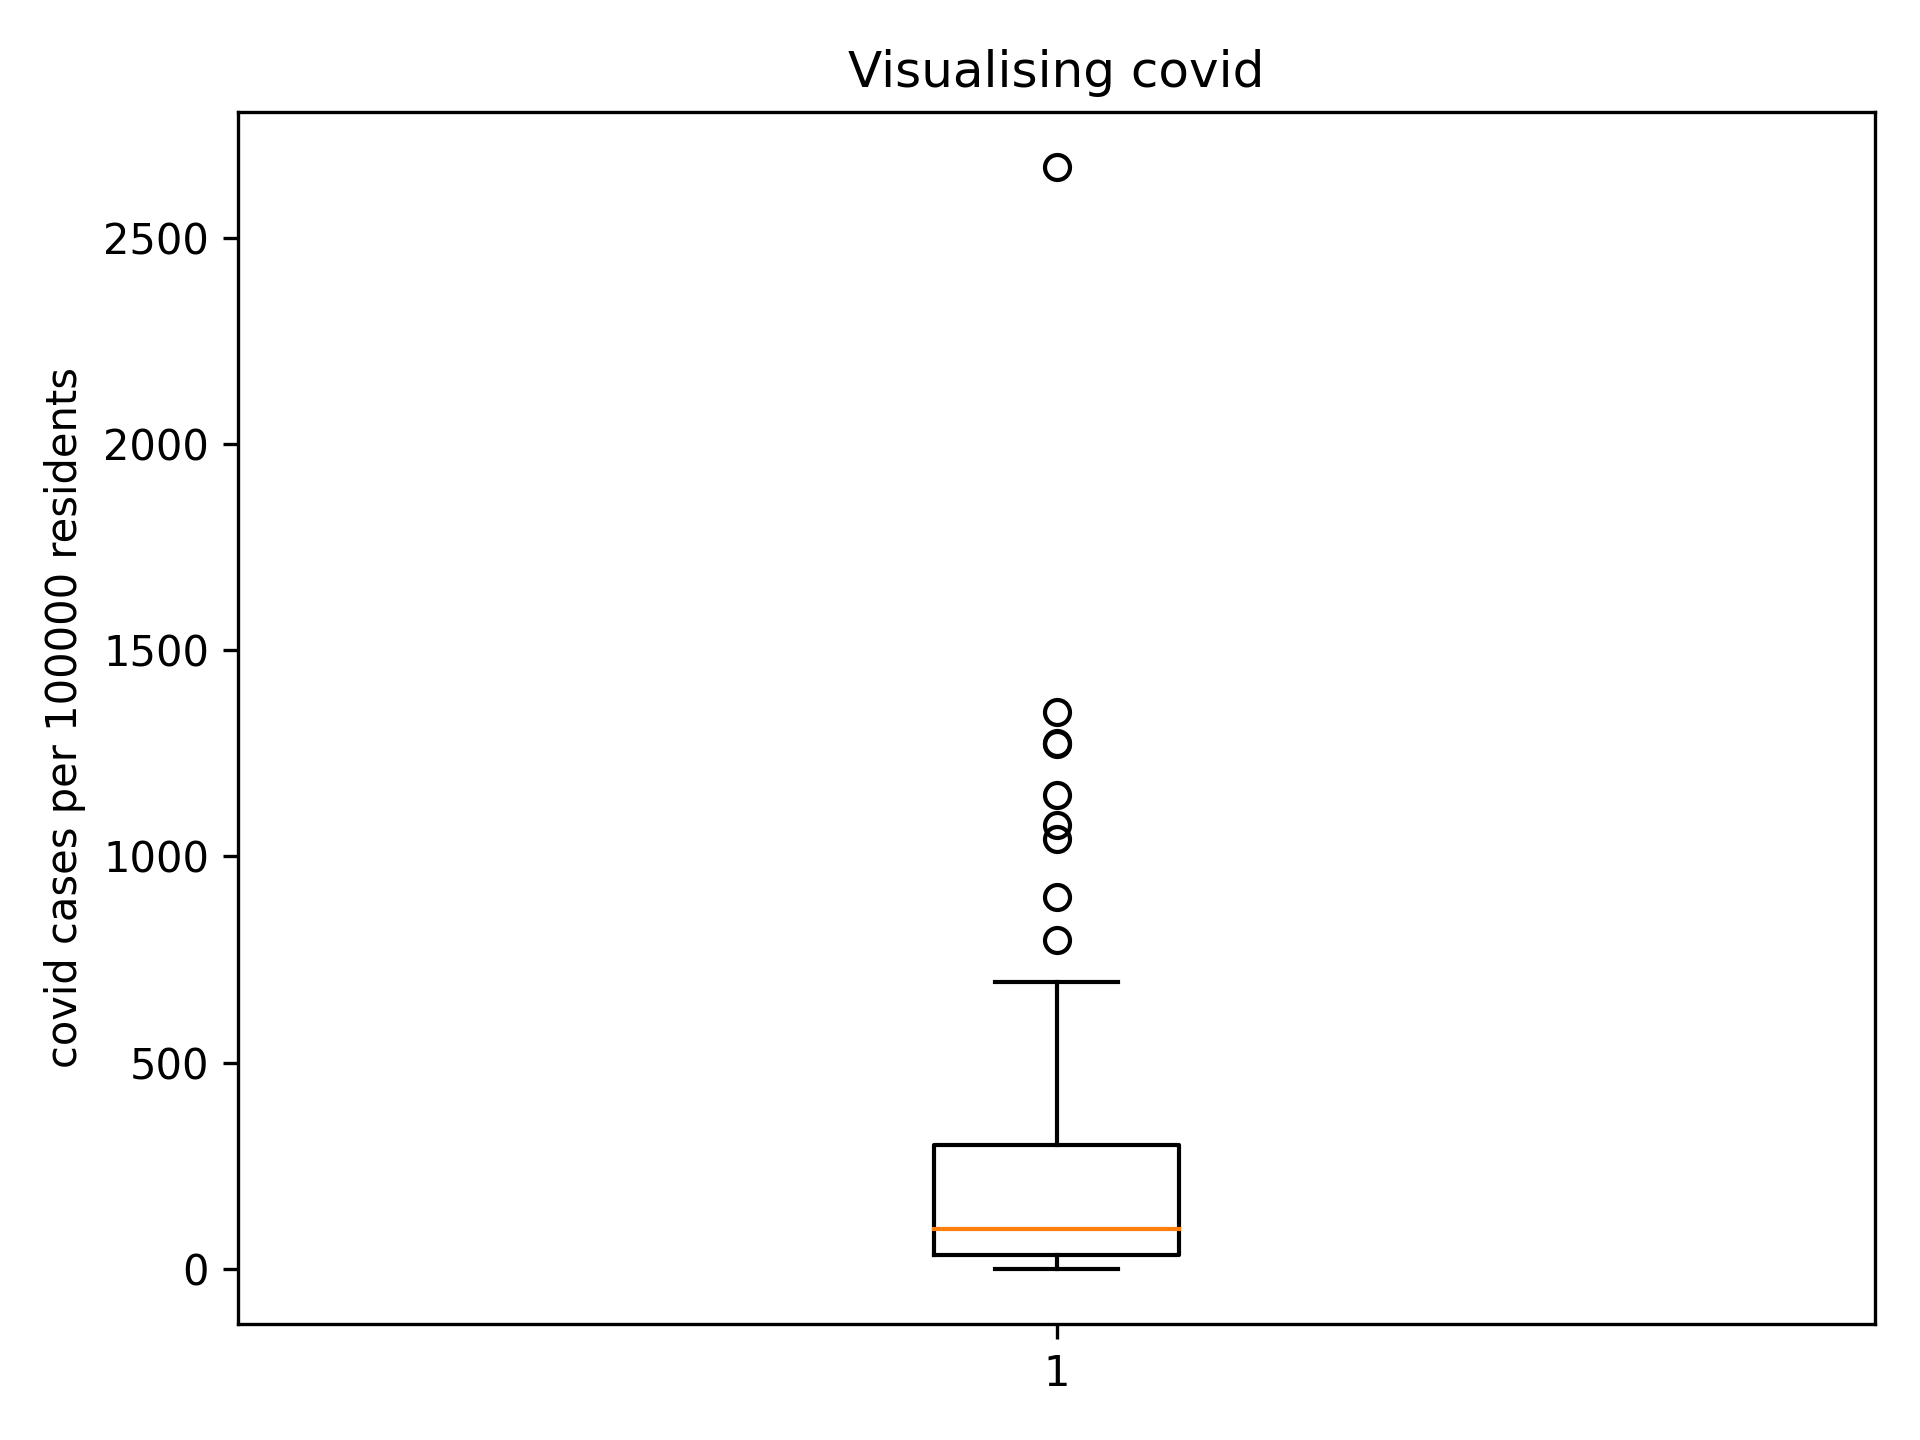
\includegraphics[width=0.4\textwidth]{graph/boxplot of covid.png}
    \caption{Boxplot for visualising COVID cases per 100000 residents}
    \label{fig:my_label}
\end{figure}
Firstly, we drew a boxplot (Figure 2), which shows the positively skewed distribution of the COVID data. We can also see from the graph that there are some outliers above 800 cases per 100000 residents. Outlier removal was therefore performed by removing those values.. 
\subsection{Scatter plots}
\begin{figure}[ht]
    \centering
    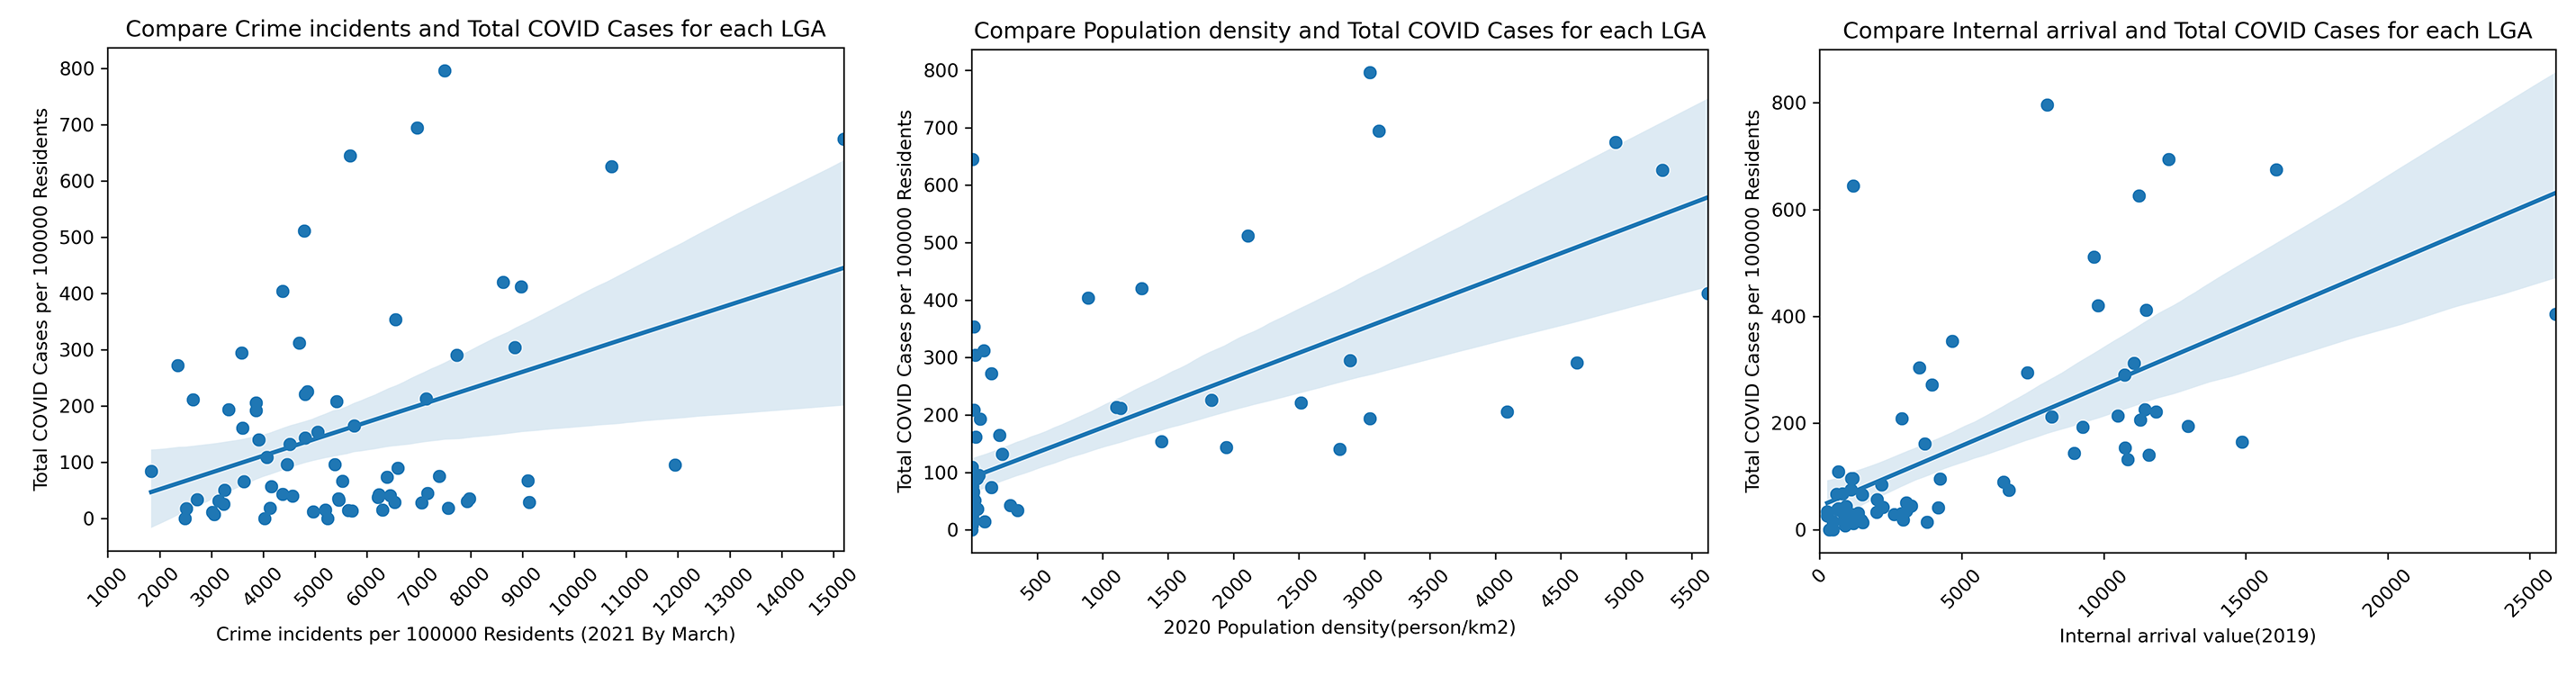
\includegraphics[width=1\textwidth]{graph/three in one scatterplot.png}
    \caption {Scatterplots for crime rate, population density and internal arrival against COVID rate by LGA}
    \label{fig:my_label}
\end{figure}
Figure 3 shows the scatter plots of crime incidents per 100000, population density and internal arrival volume plotted against numbers of COVID cases per 100000 residents. As shown, all three plots show a trend of positive correlation with different strengths. We can conclude that crime rate and COVID cases have a weak positive linear correlation, population density and internal arrival have a strong positive linear correlation with the number of COVID cases.
\begin{figure}[ht]
    \centering
    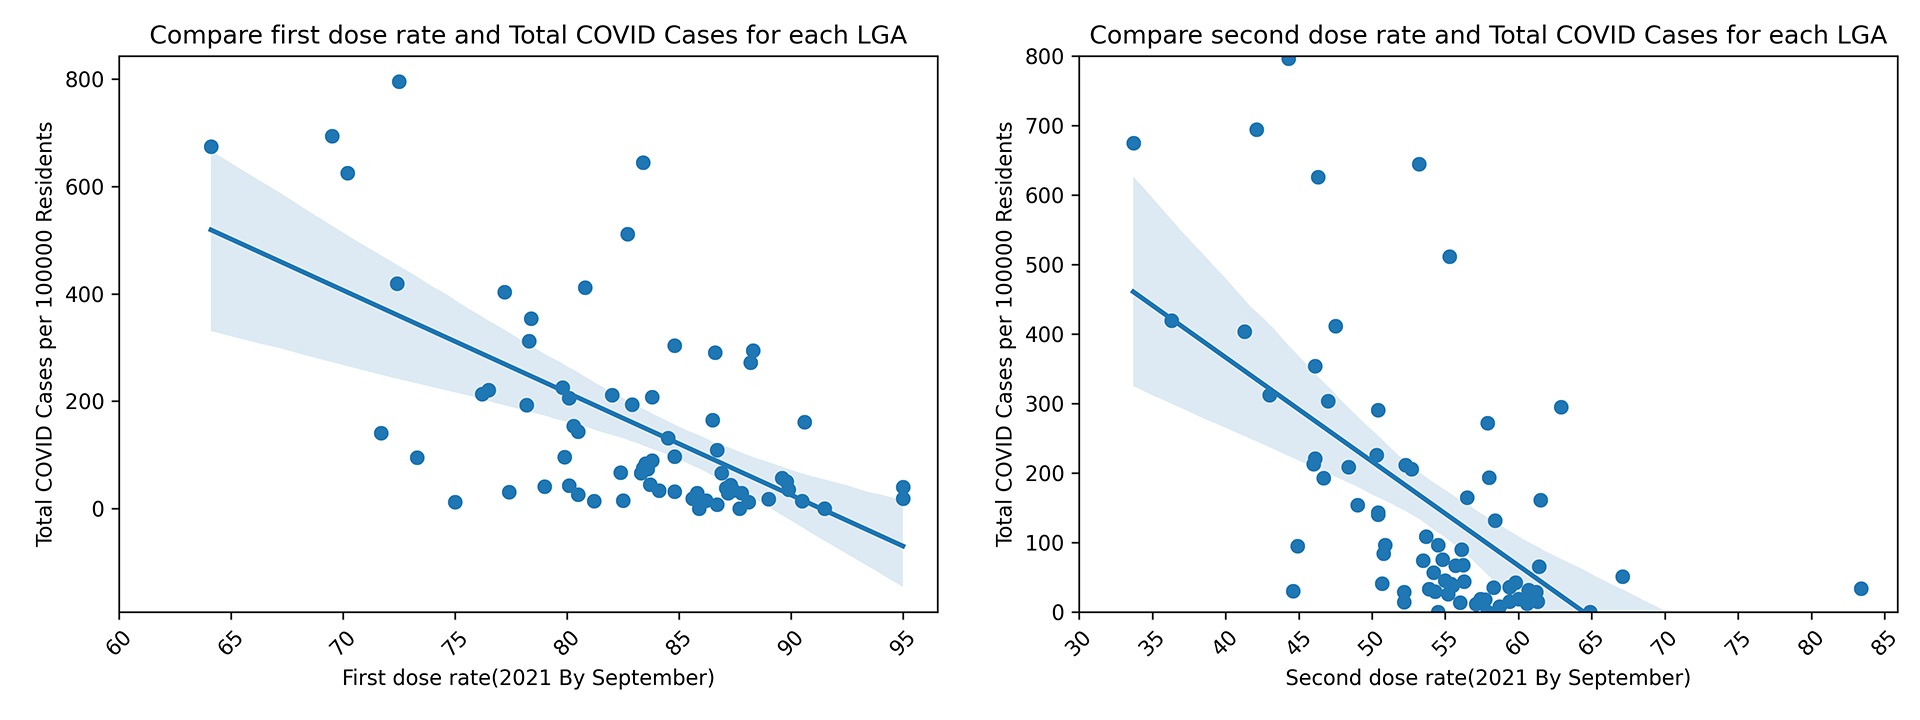
\includegraphics[width=1\textwidth]{graph/two in one scatterplot.png}
    \caption{Scatterplots for first and second dose of vaccination rate against COVID rate by LGA}
    \label{fig:my_label}
\end{figure}
\\
Figure 4 shows the scatter plots of the first dose rate of vaccine and second dose rate of vaccine. Both plots show a clear trend that the higher the rate of first dose /second dose of vaccine, the lower the number of COVID cases. We can confidently conclude that the first dose rate and second dose rate of vaccines have a strong negative linear correlation with the number of COVID cases, meaning an increase in vaccine rate of both first and second dose is highly likely to correlate to a decrease in the number of COVID cases.
\subsection{Correlation}
Normalized mutual information and Pearson r between covid rate and regional features were calculated in order to determine the correlation.(Figure 5, 6)
\begin{figure}[ht]
    \centering
    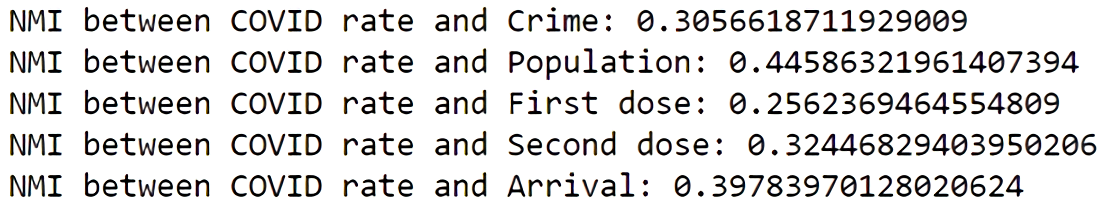
\includegraphics[width=0.7\textwidth]{captures for report/NMI value.png}
    \caption{NMI value}
    \label{fig:my_label}
\end{figure}

\begin{figure}[ht]
    \centering
    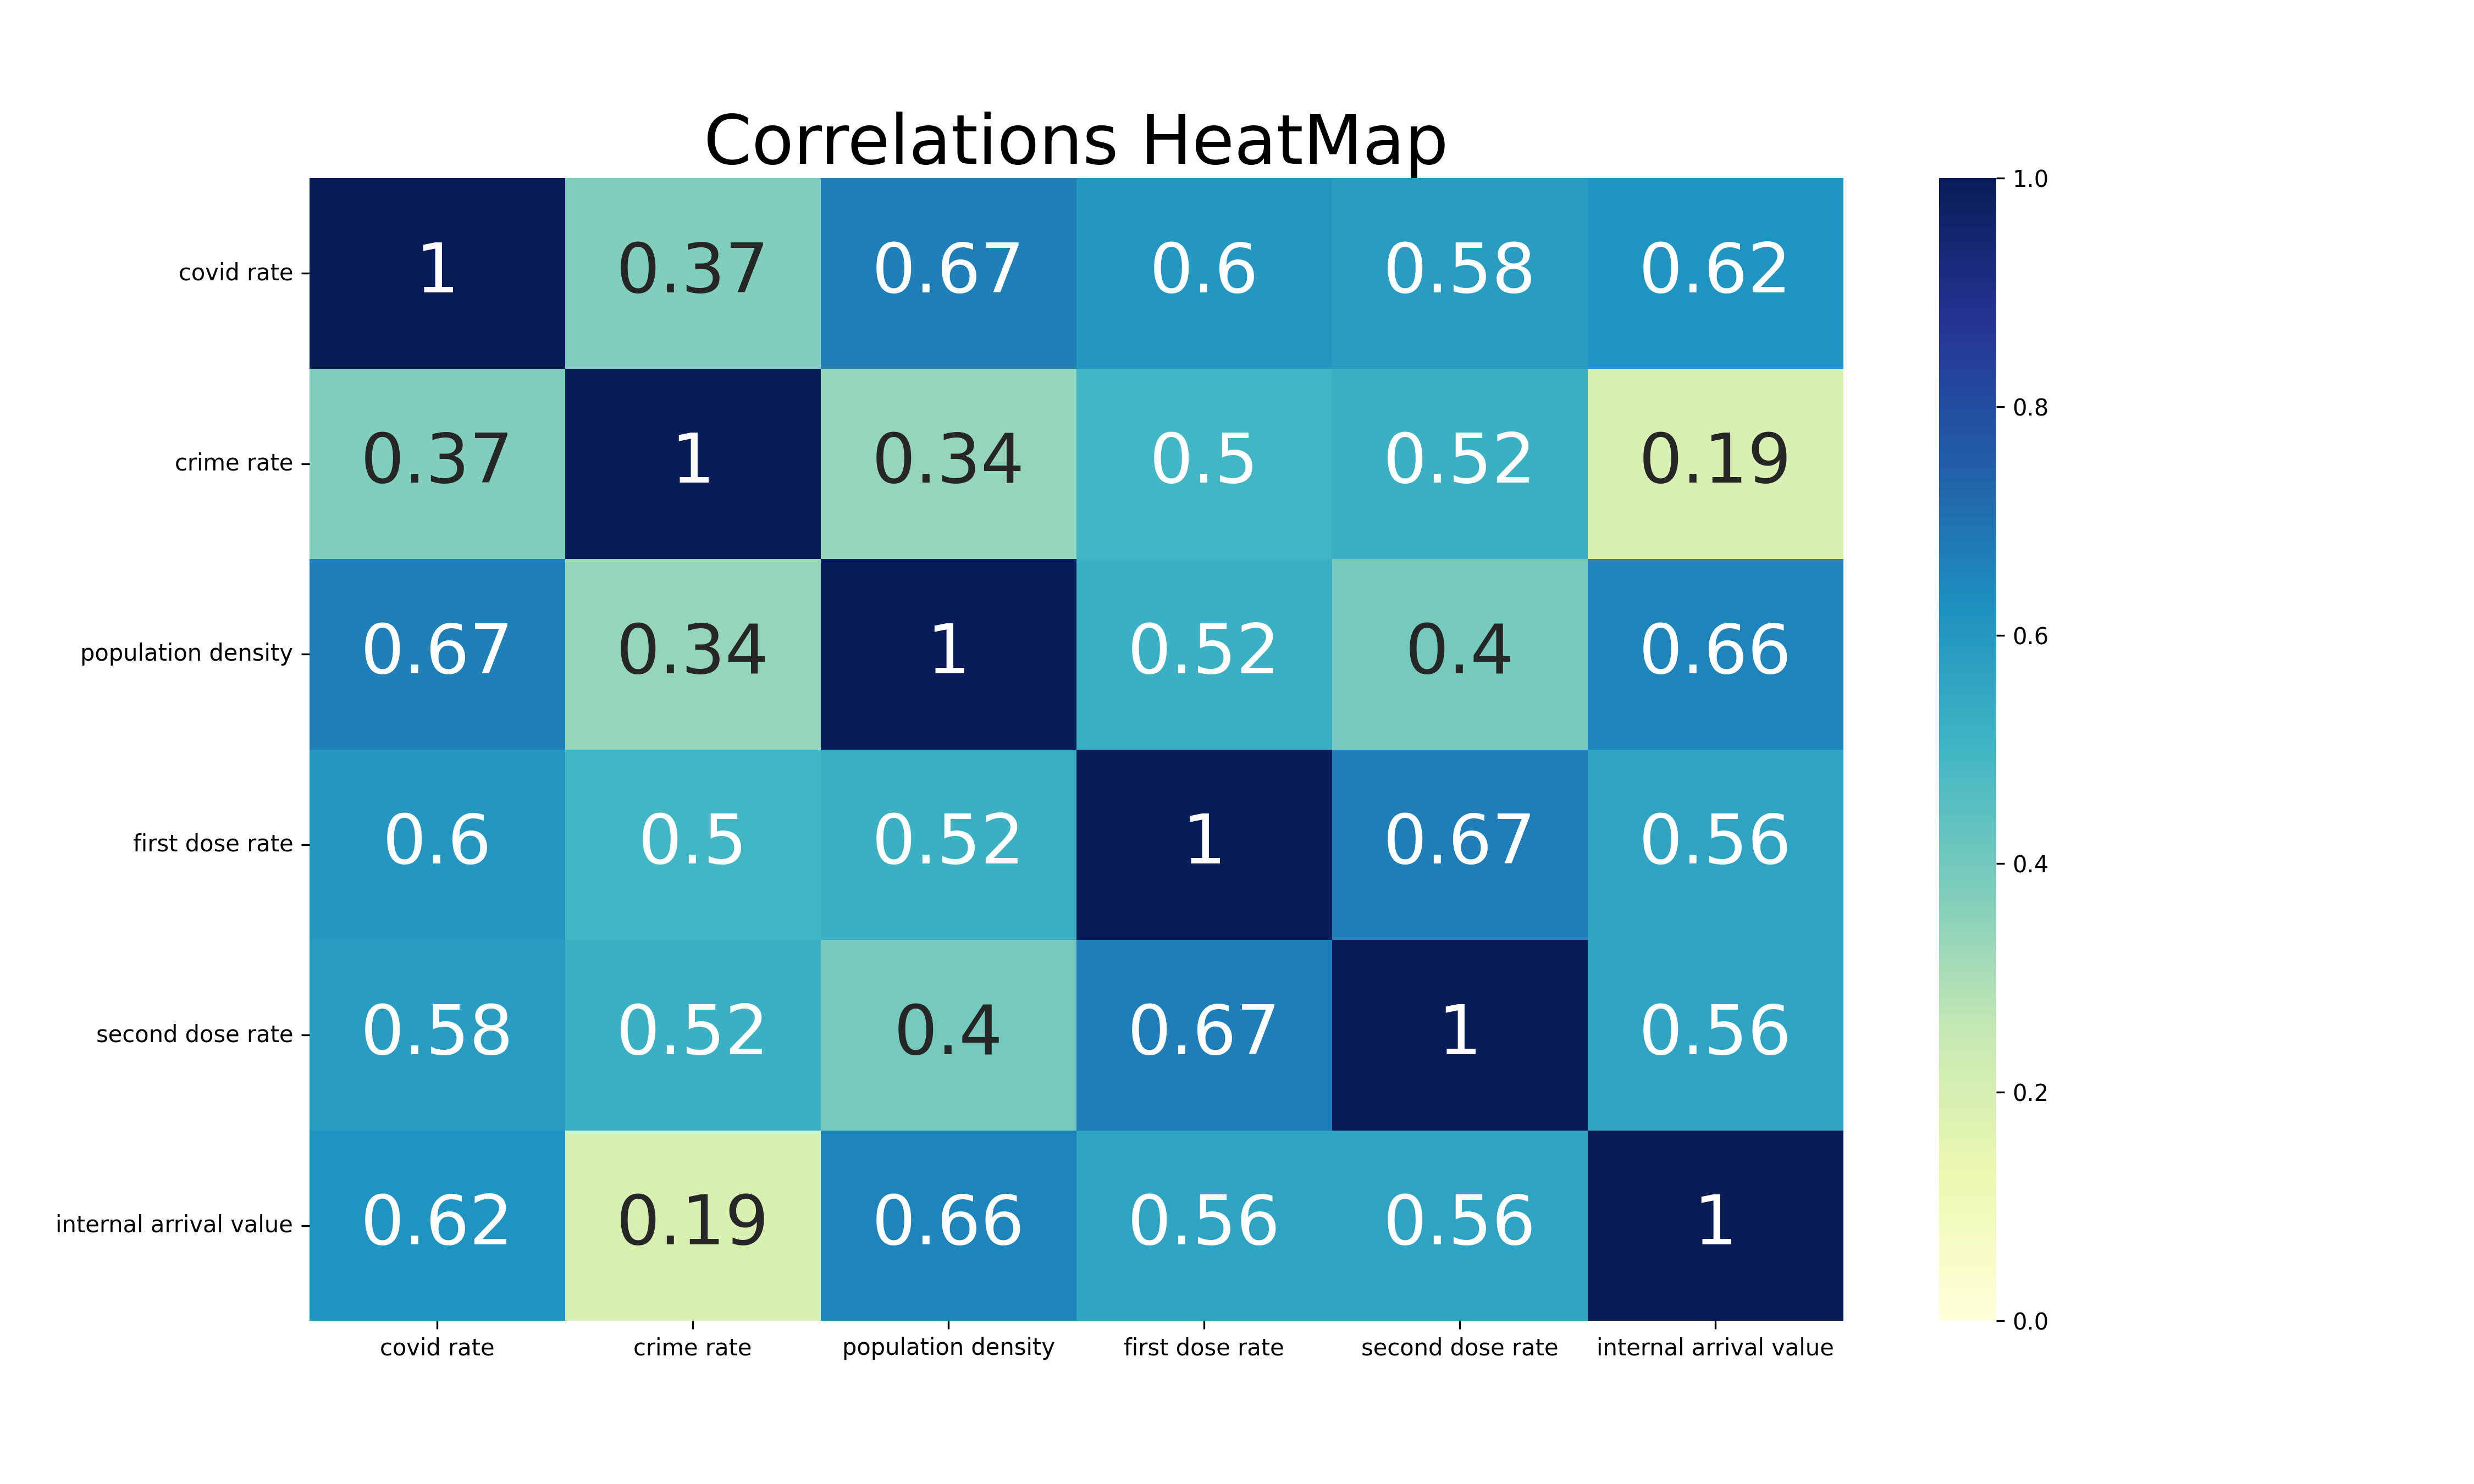
\includegraphics[width=1.2\textwidth]{graph/correlation_heatmap.png}
    \caption{Pearson correlation heatmap}
    \label{fig:my_label}
\end{figure}

The NMI correlations in Figure 5 was calculated over 8 bins with equal width. However, we discovered that the NMI value was significantly impacted by the change of binning method and number of bins. Therefore, although all the NMI we got in the case in Figure 5 were less than 0.5 which implied low correlation. We believed that the NMI was not an applicable approach for us to determine the correlation strength.\\\\\\\\\\\\
In Figure 6, we used absolute value to draw the Pearson correlation heatmap to represent the correlation degree for better visualization. The figure shows that the Pearson values between COVID rate and population density, first dose rate, second dose rate, and internal arrival are 0.67, 0.6, 0.58, 0.62, respectively. We could tell that the correlations between COVID rate and those regional features are linear and large because r values are greater than 0.5. The increase in COVID rate is highly correlated with the increase in rate of regional features. There is also a noticeable Pearson correlation between the COVID rate and crime rate (r=0.19). It suggests a weak linear correlation which means the increase in the COVID rate is weakly correlated to the increase in the crime rate. Because of high correlation, regional features except crime rate were considered to be used in the prediction model. Furthermore, considering the correlation between first dose rate and second dose rate was high (r=0.67), as well as their high degree of similarity, we excluded the second dose to ensure the model would not over-fitting or being influenced by vaccination rate too much. 


\newpage
\subsection{Classification Model}
For the classification model, firstly, we transferred the data to discrete values by 8 bins, equal width. Each bin represented 100 COVID cases. Then, we applied both KNN method and Decision Tree method. Training a set of 80\% of data and a test set of 20\% of data were used to determine the accuracy, with random state each time.
For KNN, we visualized the hyperparameter tuning based on the value of K selected (Figure 7). The graph below shows an example of how the prediction accuracy changes as the K increases. It can be seen that the KNN accuracy reached its maximum when at K = 6. However, since the graph could change subject to the change of the random training set and testing set, the optimal K varies. Therefore, we chose our K by observing a number of graphs and intuitively used k=5 as our model setup parameter.


\begin{figure}[ht]
    \centering
    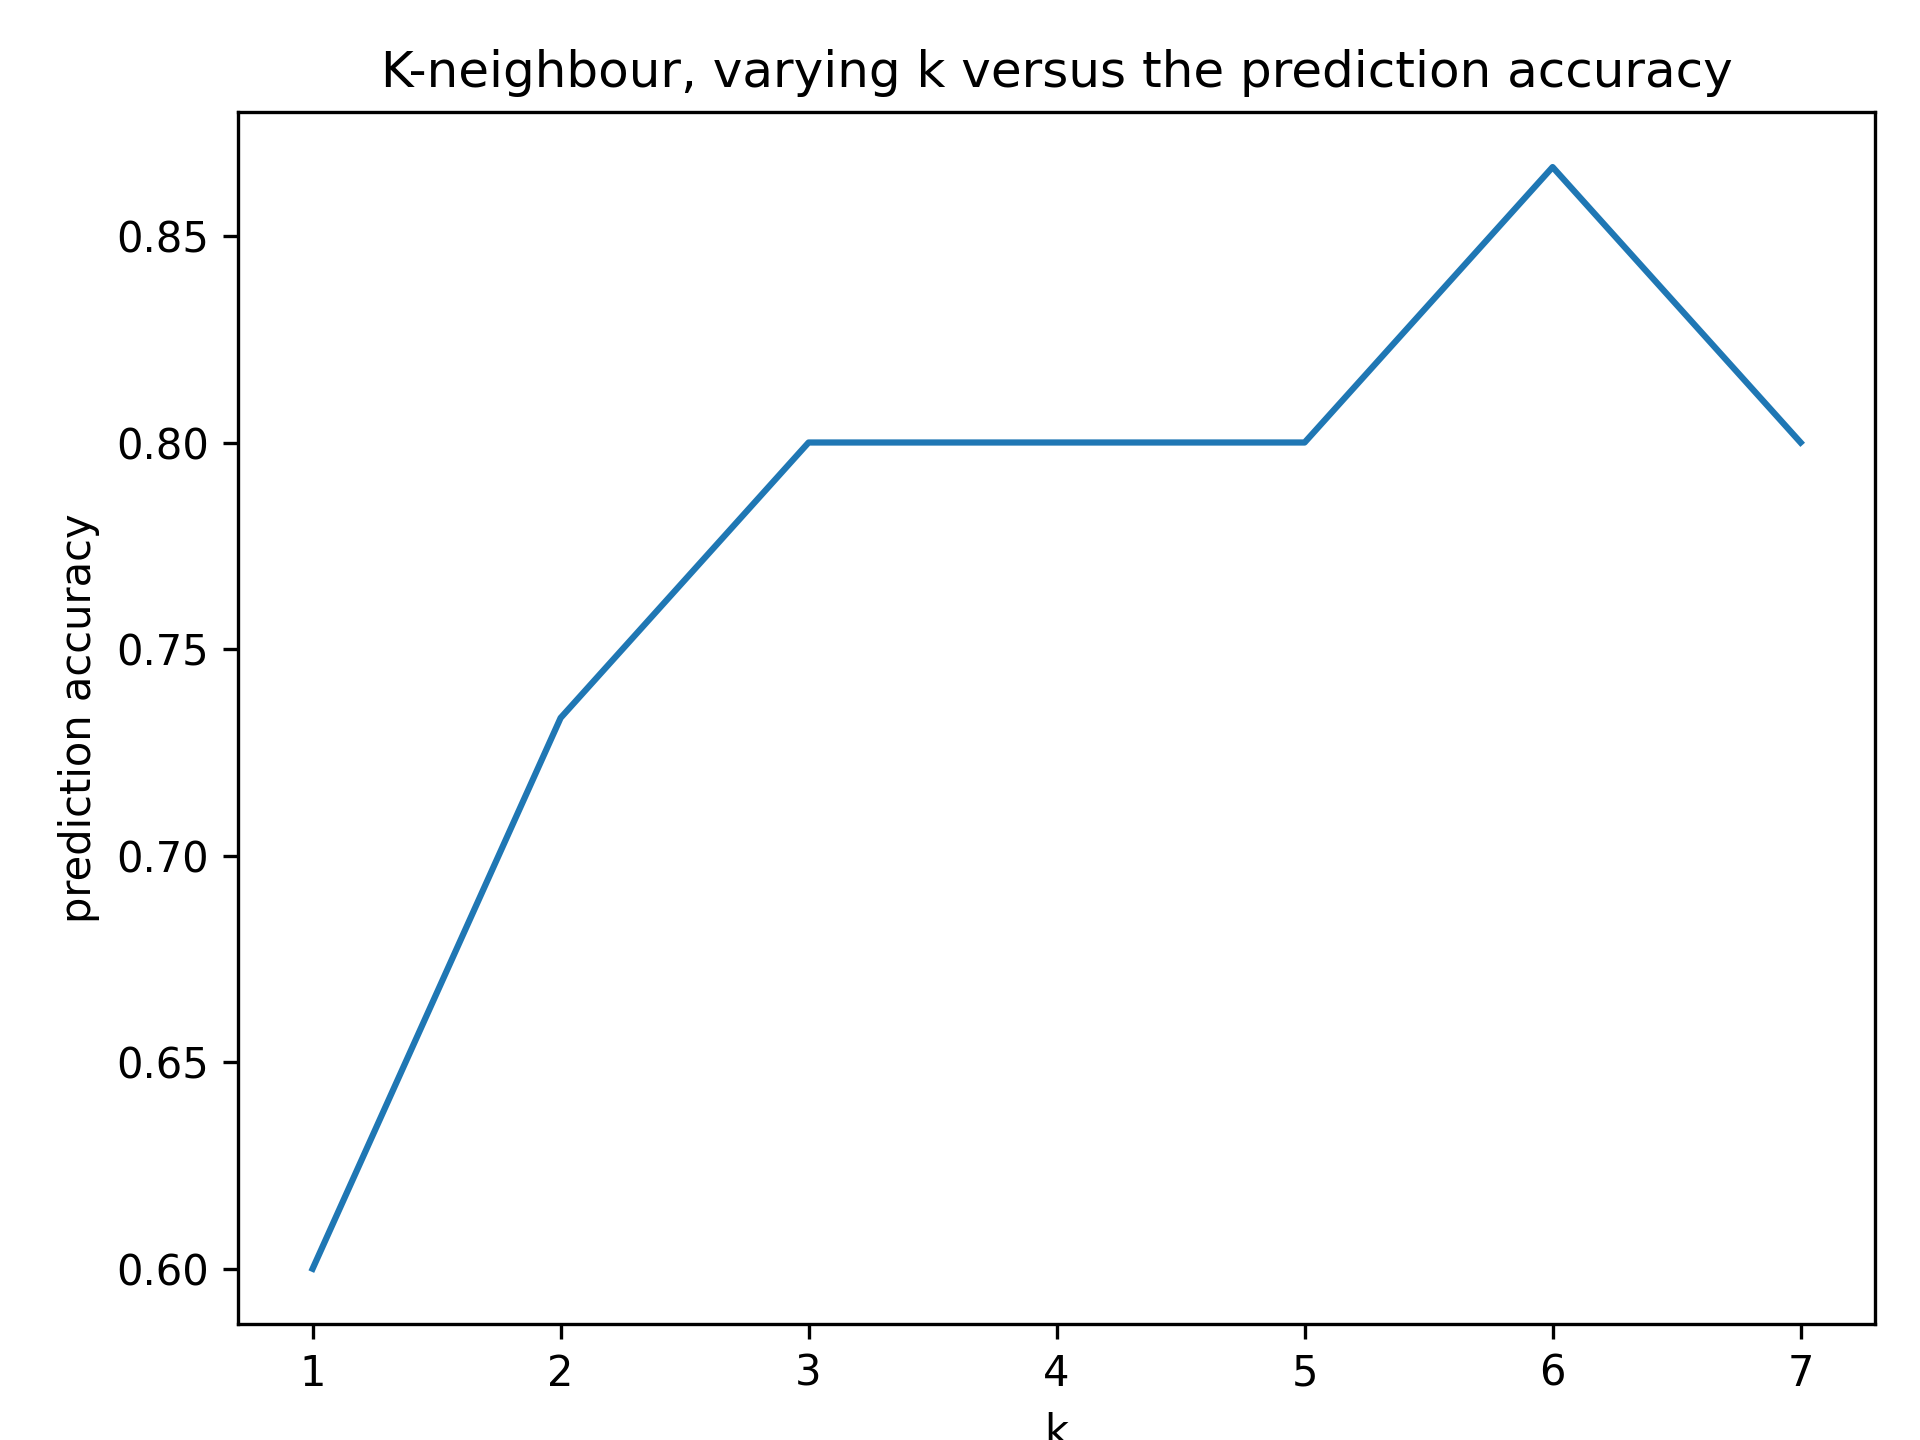
\includegraphics[width=0.5\textwidth]{graph/Sample k-NN accuracy visualization.png}
    \caption{Sample k-NN accuracy visualization, random state = 0}
    \label{fig:my_label}
\end{figure}

For the Decision Tree method, we used information gain to split the nodes (Figure 8).

\begin{figure}[ht]
    \centering
    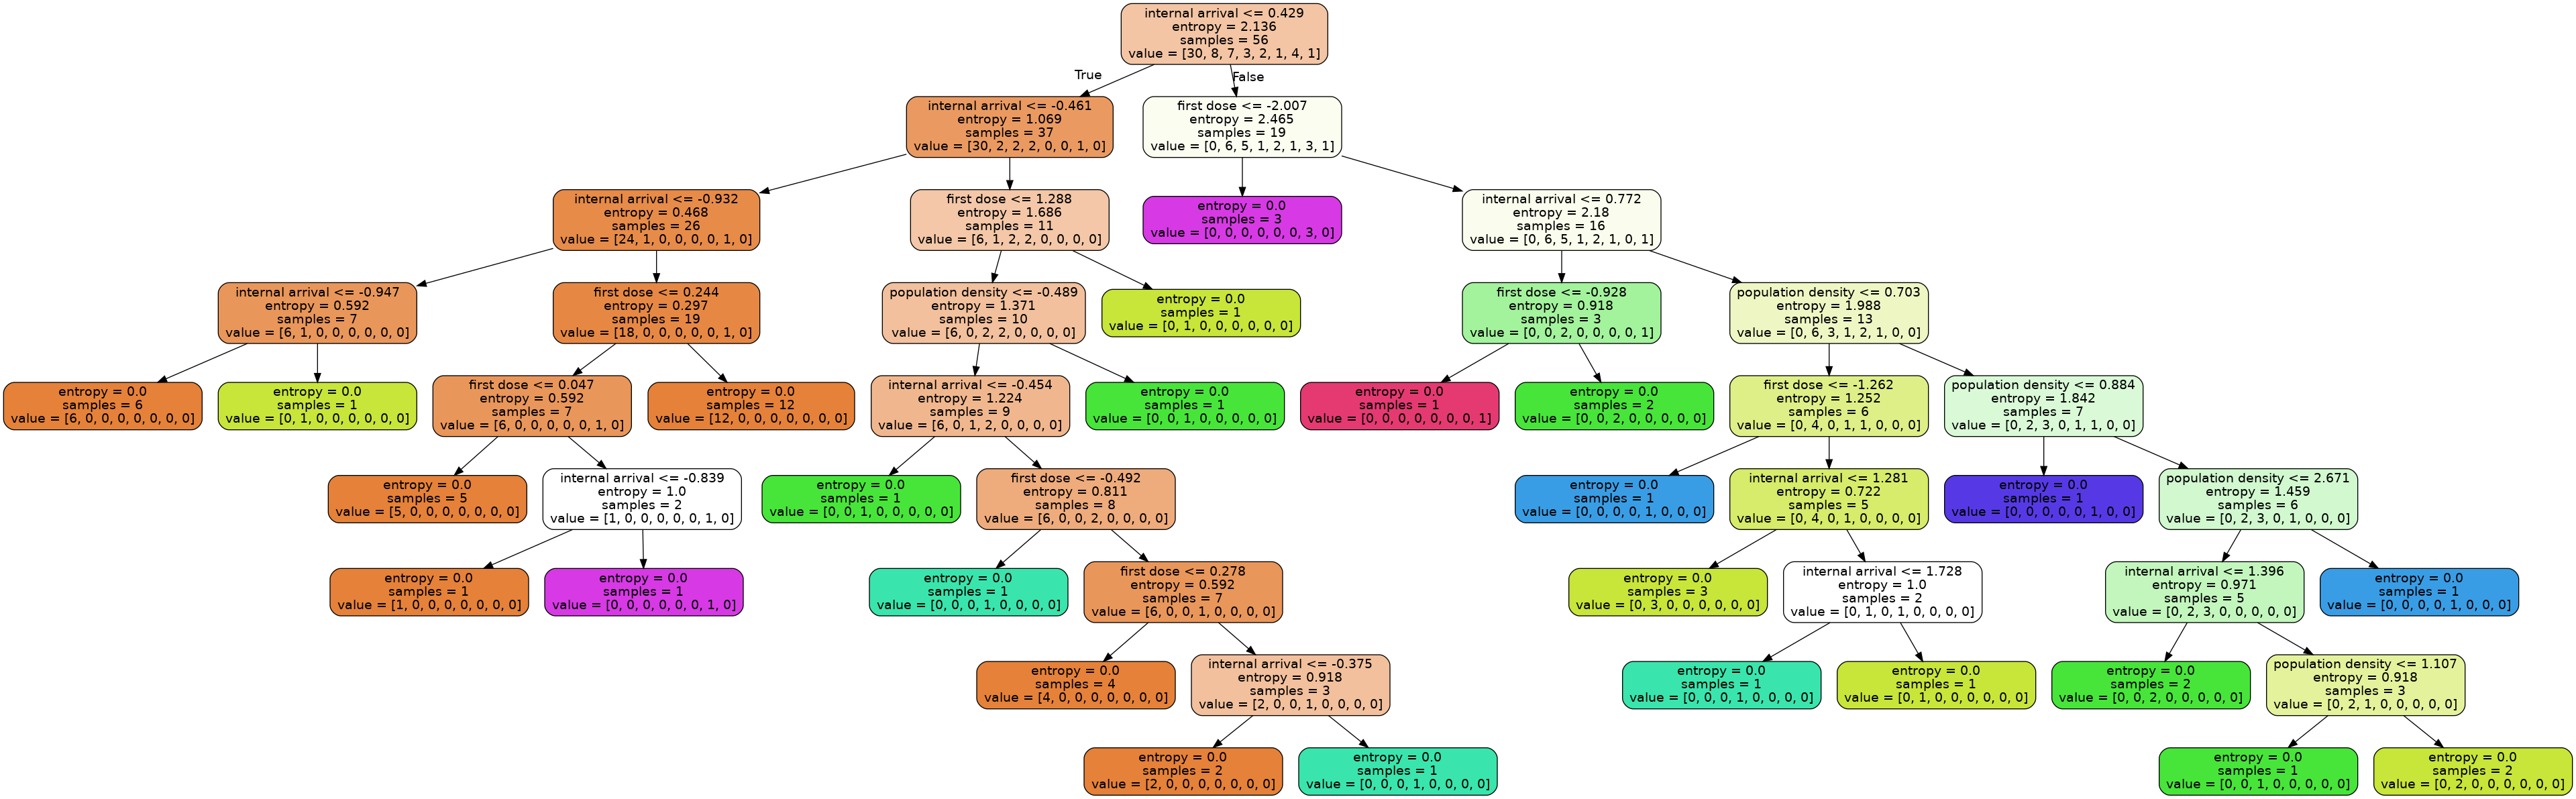
\includegraphics[width=1.05\textwidth]{graph/mytree.png}
    \caption{Decision Tree graph}
    \label{fig:my_label}
\end{figure}
Then, we started our model training and testing. 43 times of random train and tests were done for each method, with random state specified to be from 0 to 42. (Output can be found under “model\_output” folder). Two of the instances are shown in Figure 9, 10. 
\begin{figure}[ht]
    \centering
    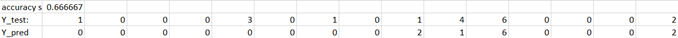
\includegraphics[width=1\textwidth]{captures for report/KNN instance.png}
    \caption{An instance of k-NN, more can be found under "model\_output/KNN.csv"}
    \label{fig:my_label}
\end{figure}

\begin{figure}[ht]
    \centering
    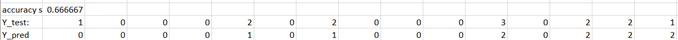
\includegraphics[width=1\textwidth]{captures for report/Decision Tree instance.png}
    \caption{Decision Tree instance, more can be found under ‘model\_output/tree.csv’ }
    \label{fig:my_label}
\end{figure}
\
\\\\\\\
After that, we calculated the average accuracy for both methods, by taking the average value of 43 tests. The average accuracy for KNN is around 0.66. The average accuracy for Decision Tree is around 0.56 (Figure 11).

\begin{figure}[ht]
    \centering
    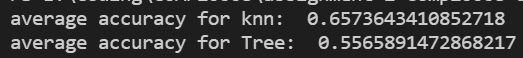
\includegraphics[width=1\textwidth]{captures for report/Average accuracy.png}
    \caption{An instance for average accuracy for KNN and Decision Tree, by running ‘model.py’}
    \label{fig:my_label}
\end{figure}
However, we were not satisfied with these two classification models. The accuracy score was significantly increased by the large number of 0 values predicted. For the non-zero values, both KNN model and decision tree model were prone to produce the prediction with considerable deviation. Hence, we believed the classification model was not applicable. We decided to stop the further evaluation of these two classification models and attempted the linear regression model.

\subsection{Linear Regression}
We conducted further modeling by linear regression. We did 43 tests with random state specified to be from 0 to 42, ensuring maximum accuracy and minimum residual. We used 80\% of data as a training set and 20\% of data as a testing set.
In order to calculate the accuracy compatible with our requirement, we implemented our own approach. We treated the prediction value as accurate, if the absolute difference between the prediction data and its test data was less than 100. Otherwise, the prediction was inaccurate. Then, the accuracy was computed as the proportion of accurate value in all the prediction values. For example, in  Figure 12, there are 11 accurate predictions and 4 inaccurate predictions. The accuracy is 11/15 = 0.73.
In general, the mean accuracy of 1000 trains is 0.70. This implies a fairly acceptable model quality. Besides, the frequency of occurrence of low (0-100) prediction is reduced, and the number of large prediction values has increased. Therefore, we believed that compared with the classification model, the regression model is more realistic and applicable.\\\\\\\\\\\\\\\\\\\\\\

\begin{figure}[ht]
    \centering
    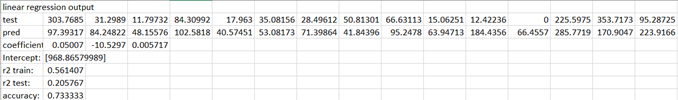
\includegraphics[width=1\textwidth]{captures for report/Linear Regression instance.png}
    \caption{An instance of Linear Regression, more can be found under ‘model\_output/lm.csv’ }
    \label{fig:my_label}
\end{figure}

Then, we did further evaluation into the regression equation we get. For each test, we calculated the coefficient of determination for both training and testing set, as well as the coefficient of Linear model and the intercept. After that, the overall mean values were calculated across the  tests (Figure 13).
\begin{figure}[ht]
    \centering
    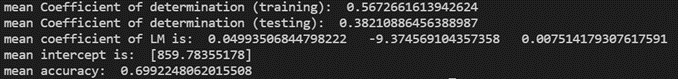
\includegraphics[width=1\textwidth]{captures for report/mean coefficient, intercept, accuracy.png}
    \caption{mean coefficient, intercept, and accuracy, by running ‘model.py’}
    \label{fig:my_label}
\end{figure}
 The coefficient of population density, first dose rate, and internal arrival is 0.050, -9.37 and 0.0075 respectively. The intercept is 859.78, Therefore, we described the regression equation as:
\\
\textbf{COVID cases per 100000 residents=859.78 + 0.050*population density -9.37*first dose rate + 0.0075 *internal arrival count}.

In addition, the R2 coefficients are 0.57 (training) and 0.38 (testing). This indicates that the variation in population density, first dose rate, and internal arrival count can explain 57\% of the COVID count in the training set, and 38\% of the COVID count in the test set.

\section{Conclusion}
The evaluation of potential linear relationships shows us a clear understanding of how change in one regional feature would affect the number of COVID cases. From Pearson correlation coefficient and the scatter plots, we can conclude that crime rate has a moderate positive linear correlation with number of COVID cases, and internal arrival and population density has a strong positive linear correlation, and vaccination rate of first dose/second dose has a strong negative correlation with number of COVID cases. The determination of Pearson R gives us a good foundation for choosing the most significant features (internal arrival and vaccine rate) for the rest of our research.
The KNN and Decision Tree classification model we built was inapplicable as it tends to produce a large number of 0 values which increases the accuracy score and fails to explain the actual COVID Trend.
The linear regression model fitted well to the dataset, with an average 0.70 accuracy which reflects the actual accuracy of prediction, eliminating the noise of 0 values compared with the classification model.
The regression model we got is:
\\
\textbf{COVID cases per 100000 residents=859.78 + 0.050*population density -9.37*first dose rate + 0.0075 *internal arrival count}


\section{Limitations}
\subsection{timeline issue}
The data we used did not exactly coincide on the timeline. For example, the last update of the crime data published by Victoria police was March, 2021 while that of the confirmed COVID case data was updated daily until the date was obtained, which was 27th September.


\subsection{model limitation}
Firstly, the amount of our training and testing data was not sufficient. After removing the outlier, there were 71 sets of data remaining. This low magnitude of data may cause inaccuracy in the model. We considered introducing more datasets in different timelines. However, this was practically unreachable as the four regional features had significant statistical timeline inconsistency. For example, the data for the population density, internal arrival and crime rate were published every 6 or 12 months. The vaccination rate and COVID rate were published daily. This was one of the main reasons why our project focused more on the analysis of a certain date (27/09/2021, when the data for COVID Cases was collected), instead of a certain time frame. Hence, the available magnitude of data was limited, therefore our model may have omission.\\
We selected the model input features (population density, internal arrival, and first dose rate) because they all have high correlation with the COVID rate. However, these selection criteria were not theoretically rigorous. For further evaluation, several feature selection methods such as Wrapper Method, Greedy Method, Chi Squared Feature Selection and Principal Component Analysis can be used.




\section{Links to Data Sets}
COVID confirmed cases: https://discover.data.vic.gov.au/dataset/all-victorian-sars-cov-2-cases-by-local\\-government-area-postcode-and-acquired-source/resource/890da9b3-0976-4de3-8028-e0c22b9a0e09 

COVID vaccination rate: https://covidlive.com.au/report/vaccinations-by-lga/vic

Internal arrival: 
https://stat.data.abs.gov.au/Index.aspx?QueryId=916

Regional population: 
https://www.abs.gov.au/statistics/people/population/regional-population/
 
Crime incidents: 
https://www.crimestatistics.vic.gov.au/crime-statistics/latest-crime-data-by-area



\end{document}
